\section{Finetuning Projects the Pretrained Manifold onto Time Series}
\label{sec:finetuning}


\subsection{The Weight Changes are Low-Rank}
\label{sec:lora}

% LoRA vs IO-only vs full finetuning comparison
% Key point: LoRA with small rank captures most of the transfer benefit,
% proving only a low-rank perturbation of the weights is needed.

% ── TABLE: Finetuning regime comparison ──
\begin{table}[h]
\centering
\caption{Finetuning regime comparison on GiftEval ND[0.5]. TODO: fill from Alexis's experiments.}
\label{tab:lora}
\begin{tabular}{lccc}
\toprule
Method & Params changed & ND[0.5] & \% of full FT \\
\midrule
Full finetuning     & 100\%  & TODO & 100\%  \\
LoRA ($r=16$)       & TODO\% & TODO & TODO\% \\
LoRA ($r=4$)        & TODO\% & TODO & TODO\% \\
IO-only (emb + head)& TODO\% & TODO & TODO\% \\
Random init (full)  & 100\%  & TODO & ---    \\
\bottomrule
\end{tabular}
\end{table}

\paragraph{Interpretation.} Only a low-rank perturbation of the pretrained weights is needed to adapt the model from language to time series. This means the bulk of the pretrained computation is preserved---finetuning adjusts a small subspace of directions.


\subsection{Finetuning Selects Useful Directions}
\label{sec:dimensionality}

% Table moved to appendix (Table~\ref{tab:effrank} and Table~\ref{tab:alignment})

% ── FIGURE: Effective rank + Subspace alignment across layers ──
\begin{figure}[!ht]
\centering
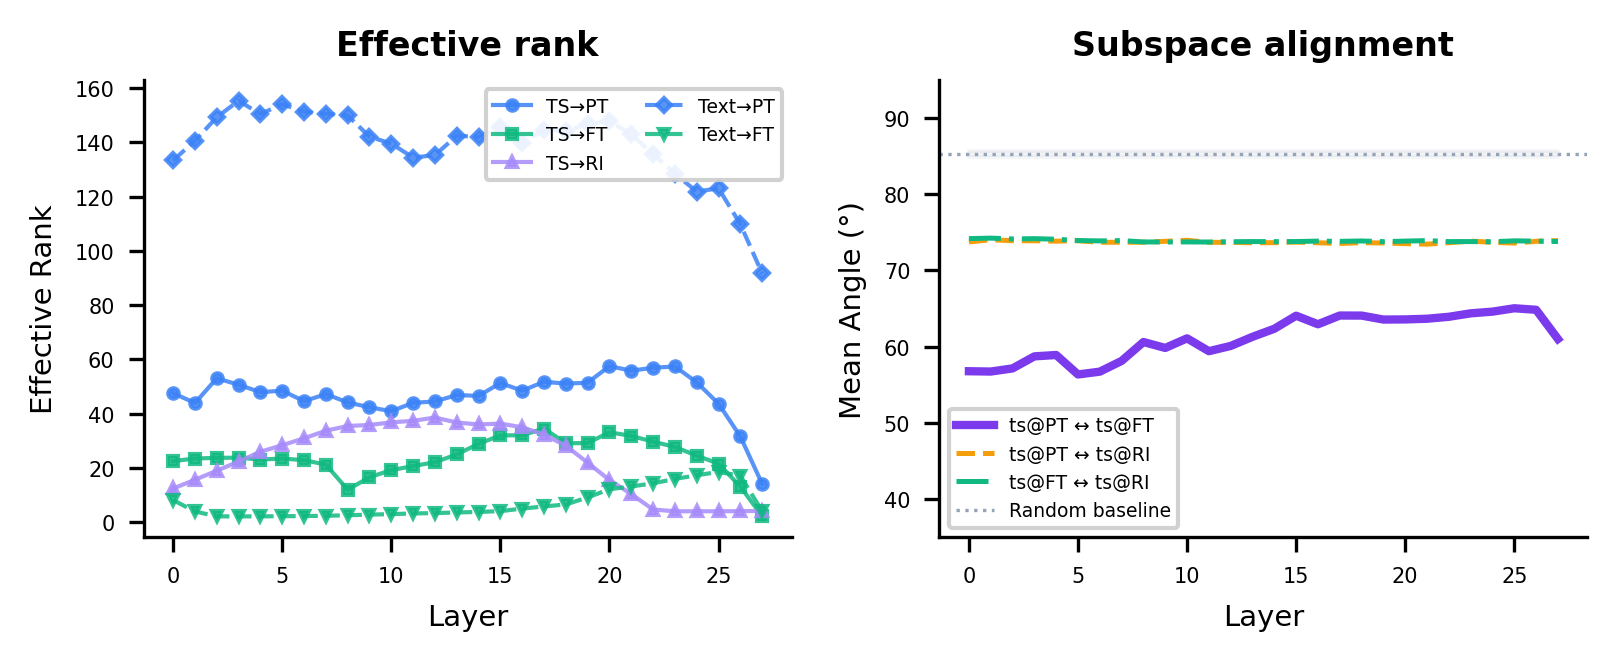
\includegraphics[width=0.95\textwidth]{figures/sec5/fig_geometry.png}
\caption{\textbf{Geometric evidence for direction reuse.} \textbf{(Left)} Effective rank across layers. FT compresses TS representations to $\sim$12 dimensions (green solid), far below PT's $\sim$44 (blue solid) and RI's $\sim$35 (purple solid). Text$\to$FT collapses to $\sim$2.5 (catastrophic forgetting). \textbf{(Right)} Subspace alignment: mean principal angle between top-10 PCs. ts@PT$\leftrightarrow$ts@FT (purple) stays well below the random baseline (85.3$^\circ$), confirming FT reuses PT's directions. Tables~\ref{tab:effrank} and~\ref{tab:alignment} in Appendix.}
\label{fig:geometry}
\end{figure}

\paragraph{Catastrophic forgetting as geometric compression.}
Text$\to$FT collapses to effective rank 2.5 (from 150 in PT). Finetuning traded $\sim$140 text-useful dimensions for $\sim$12 TS-useful dimensions.

\paragraph{Method: effective rank across training.}
To track how representational geometry evolves during training, we compute the effective rank of hidden-state covariance matrices at every saved checkpoint. For each checkpoint and each of the 28 transformer layers, we pass 10{,}000 time-series windows (length 512, drawn from the GiftEval validation split) through the model, collecting hidden states at every position except position~0 (excluded to avoid the attention-sink artifact). For FT and FT\textsubscript{IO} we additionally pass 10{,}000 WikiText-103 sequences to track text representation quality.

At each layer we accumulate the centered covariance matrix $\Sigma = \frac{1}{N}\sum_i \mathbf{h}_i \mathbf{h}_i^\top - \bar{\mathbf{h}}\bar{\mathbf{h}}^\top$ in float64 over all $N$ hidden-state vectors ($N \approx 130{,}000$ per batch), then compute its eigendecomposition. The effective rank is $\mathrm{erank}(\Sigma) = \exp\!\bigl(-\sum_i p_i \log p_i\bigr)$, where $p_i = \lambda_i / \sum_j \lambda_j$ are the normalized eigenvalues~\citep{roy2007effective}. This equals 1 when all variance concentrates on a single direction and equals the ambient dimension $d$ when variance is uniformly spread.

We evaluate all checkpoints for three training regimes: FT (full finetuning from PT, 15 checkpoints from step 1 to 10{,}000), FT\textsubscript{IO} (input/output layers only, 17 checkpoints from step 1 to 33{,}000), and RI (randomly initialized, 14 checkpoints from step 1 to 8{,}192). The pretrained model (PT) serves as a fixed baseline. Checkpoints are processed 4 at a time across 4 GPUs.

\begin{figure}[!ht]
\centering
\begin{subfigure}[t]{0.48\textwidth}
\centering
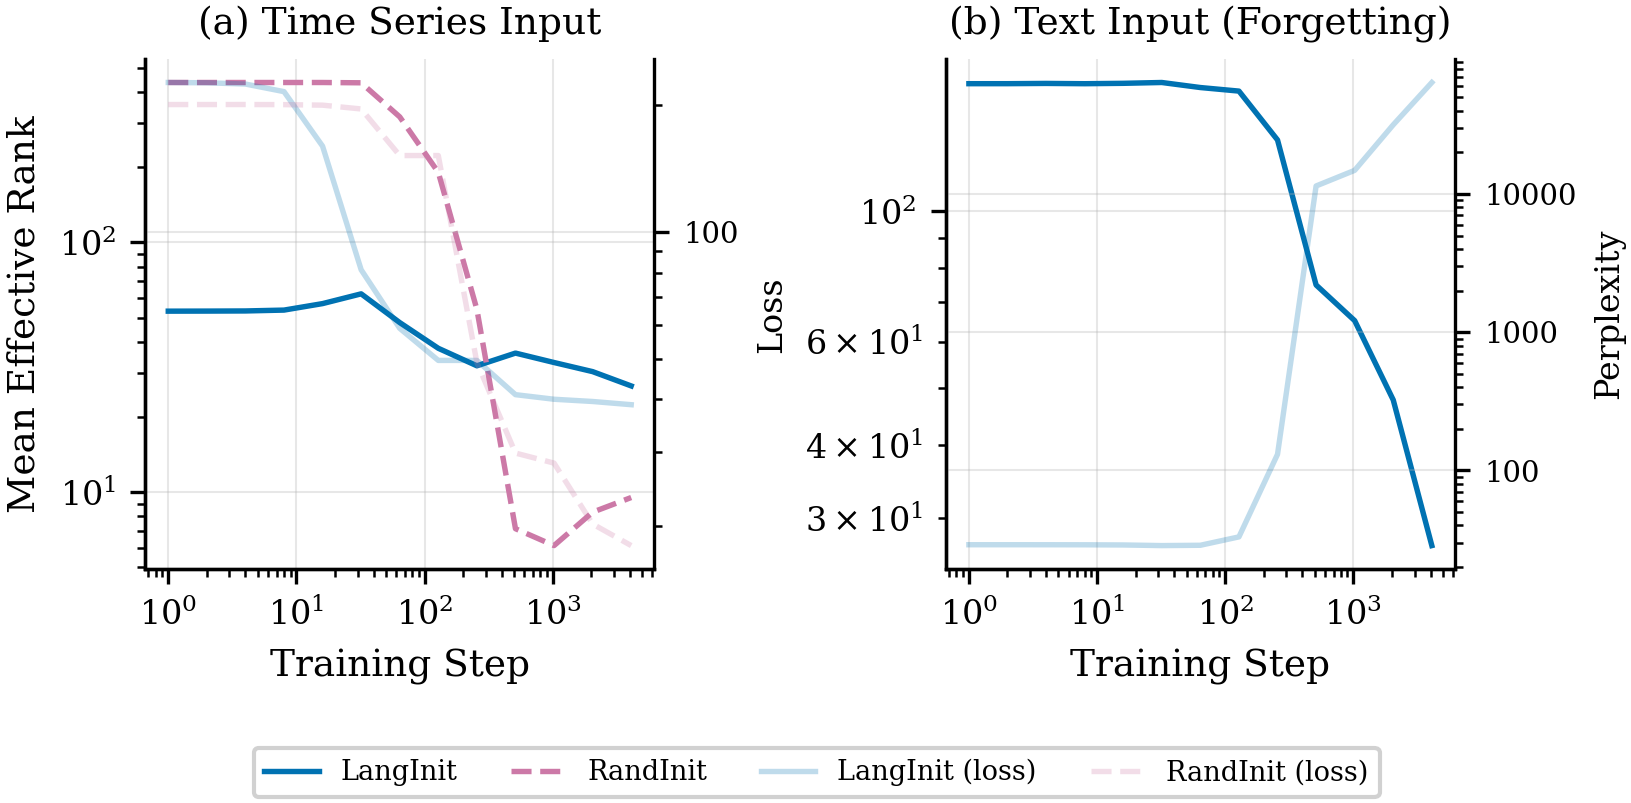
\includegraphics[width=\textwidth]{figures/sec5/fig_erank_trajectory.png}
\label{fig:erank_trajectory}
\end{subfigure}
\hfill
\begin{subfigure}[t]{0.48\textwidth}
\centering
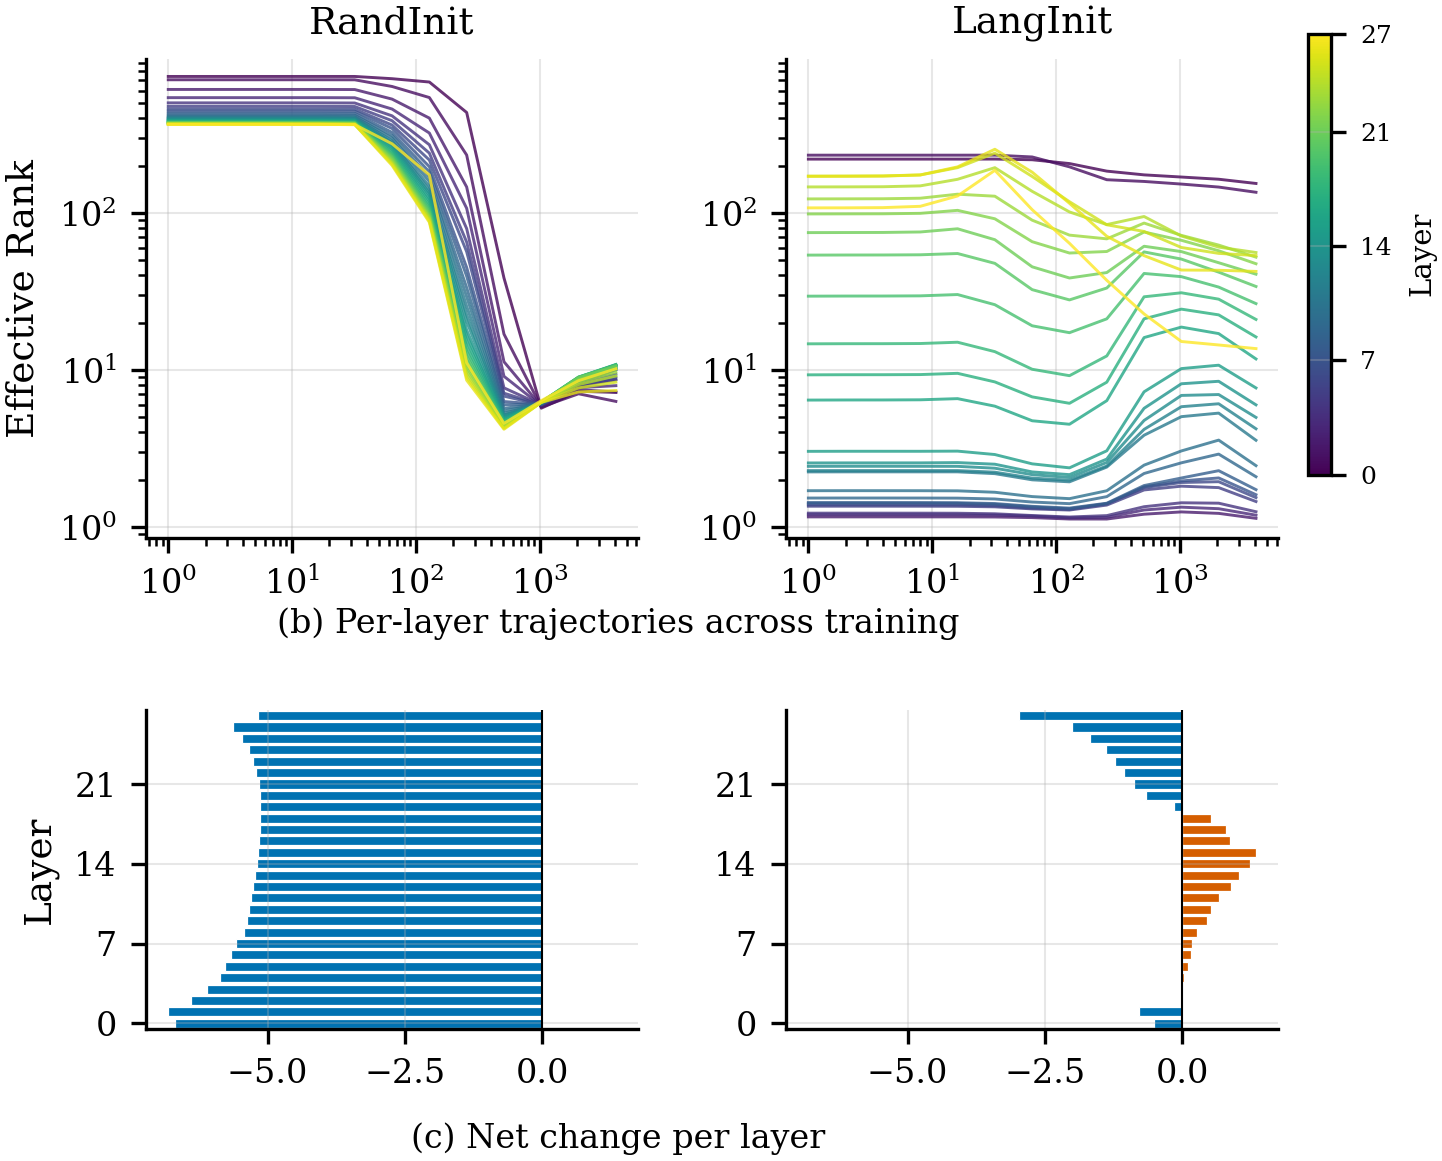
\includegraphics[width=\textwidth]{figures/sec5/fig_erank_layers.png}
\label{fig:erank_layers}
\end{subfigure}
\caption{\textbf{Effective rank dynamics during training.} \textbf{(a)}~Mean effective rank across all 28 layers. Left: on time-series input, RandInit starts near-isotropic ($\sim$440) and collapses to $\sim$10 within 500 steps; LangInit declines more gradually from the pretrained baseline ($\sim$50) to $\sim$27. Transparent lines show CRPS loss on a secondary axis. Right: on text input, LangInit's effective rank drops from $\sim$165 to $\sim$25 (85\% reduction) while perplexity rises, confirming catastrophic forgetting. \textbf{(b)}~Per-layer trajectories (each line = one of 28 layers, colored by depth). RandInit layers collapse as a tight bundle; LangInit middle layers ($\sim$8--17) \emph{increase} their effective rank while early and late layers decrease. \textbf{(c)}~$\log_2$ change (final/initial) per layer. Orange = gained rank; blue = lost. RandInit is uniformly negative ($-5$ to $-7$, i.e., 32--128$\times$ reduction). LangInit layers 10--17 show positive change (up to $+1$ log$_2$ = $2\times$ increase)---finetuning redistributes capacity from the network's periphery to its core.}
\label{fig:erank_dynamics}
\end{figure}


\subsection{Reuse vs.\ Reinvention: LangInit and RandInit Find Different Solutions}
\label{sec:reuse_vs_reinvent}

\paragraph{Method.}
To probe how each model geometrically encodes temporal structure, we pass synthetic waveforms through the network and visualize hidden-state trajectories via 2D PCA. We generate five inputs of length 512: a sine wave (period~64), a square wave (period~64), a sawtooth wave (period~64), a two-frequency signal ($\sin(2\pi t/64) + 0.5\sin(2\pi t/17)$), and a linear trend with oscillation ($t/T + 0.3\sin(2\pi t/80)$). Each input is independently $z$-score normalized, clipped to $[-5, 5]$, and uniformly binned into 1024 tokens. The tokenized sequence is passed through the model, and we extract hidden states at the target layer. PCA is fitted independently per model--input pair, since the models occupy different regions of representation space. The first 5 positions are excluded to avoid the attention-sink artifact. Trajectories are colored by input phase (position mod period / period) to reveal periodic structure. Full per-layer breakdowns for all 28 layers are provided in Figures~\ref{fig:pca_grid_ft} and~\ref{fig:pca_grid_ri} in the Appendix.

% ── FIGURE: Sine layer evolution + coherence evolution ──
\begin{figure}[!ht]
\centering
\begin{minipage}[t]{0.42\textwidth}
\centering
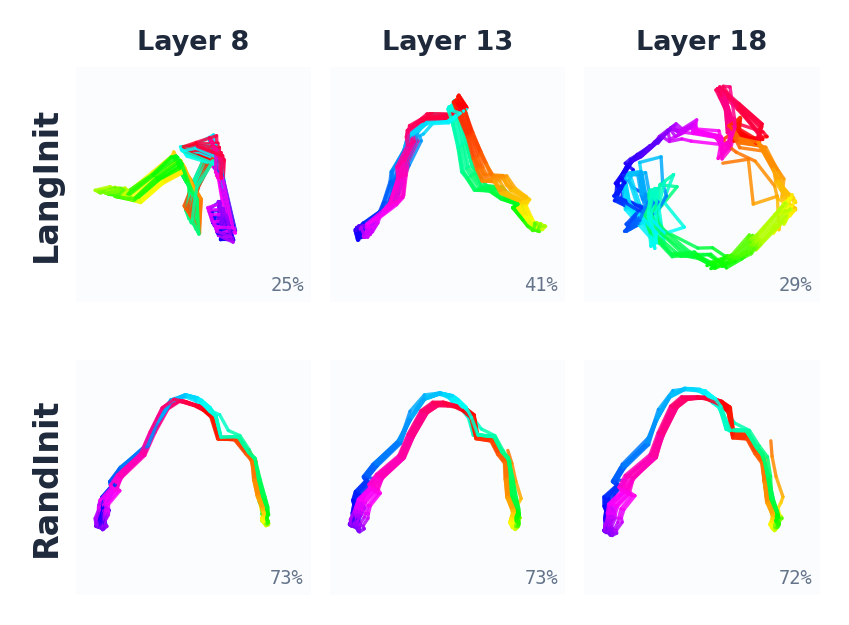
\includegraphics[width=\textwidth]{figures/sec5/fig_sine_evolution.png}
\end{minipage}%
\hfill
\begin{minipage}[t]{0.56\textwidth}
\centering
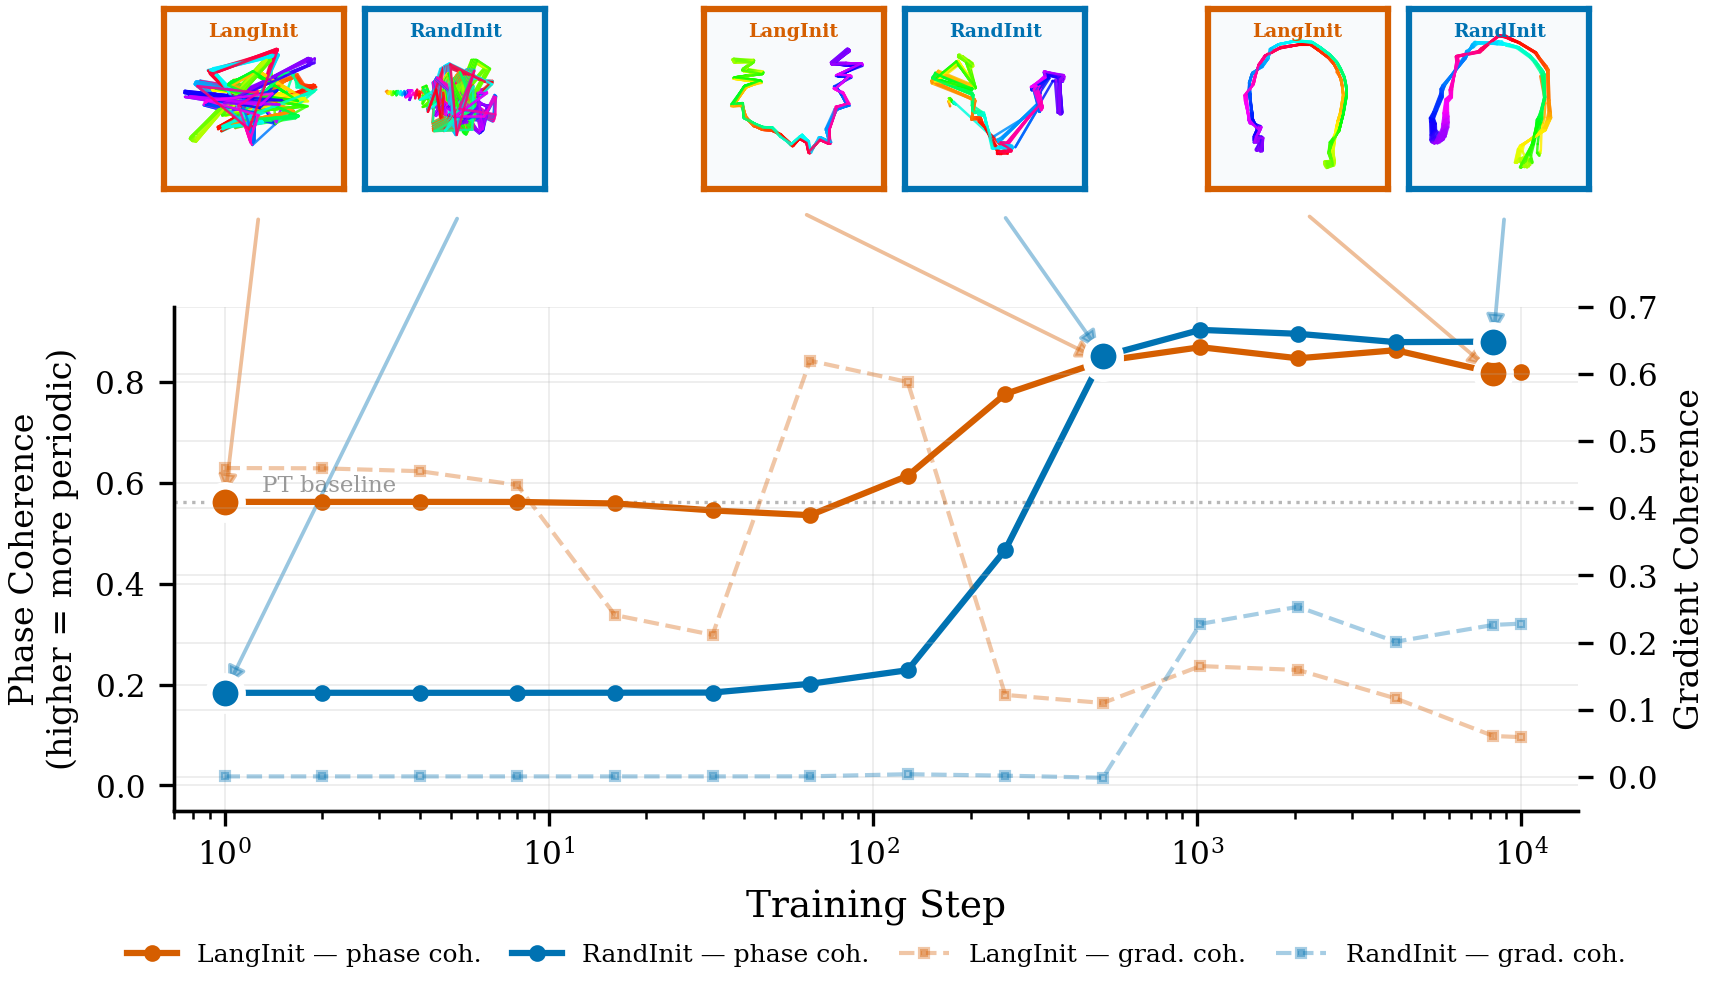
\includegraphics[width=\textwidth]{figures/sec5/fig_coherence_evolution.png}
\end{minipage}
\caption{\textbf{Left: Sine wave representations across layers.} A sine wave (period~64) passed through LangInit (top) and RandInit (bottom) at layers 8, 13, and 18, shown as 2D PCA colored by input phase. RandInit produces clean arcs at every layer (72--73\% PCA variance); LangInit produces complex, layer-varying loops (25--41\%).
\textbf{Right: Phase and gradient coherence across training.} Phase coherence (solid; $1 - \text{same-phase} / \text{all-pair distance ratio}$, higher = more periodic) and gradient coherence (dashed) at Layer~13. Insets show t-SNE of hidden states at steps 1, 512, and 8192. LangInit inherits periodic structure from pretraining and starts high; RandInit starts near zero and undergoes an abrupt phase transition around step~256--512 where gradient coherence simultaneously spikes, indicating that the model discovers periodic geometry at the same moment it begins aligning gradients across the time series.}
\label{fig:sine_evolution}
\end{figure}

Figure~\ref{fig:sine_evolution} (left) shows this contrast for a single sine wave across three representative layers. RandInit converges to a uniform, clean arc at every layer, with 72--73\% of variance explained by just two principal components. LangInit produces complex, layer-specific loops with only 25--41\% PCA variance---the periodic structure is distributed across many more dimensions, reflecting the richer geometry inherited from pretraining. Figure~\ref{fig:sine_evolution} (right) tracks how this geometry emerges during training: LangInit inherits high phase coherence from the start, while RandInit undergoes a sharp phase transition around step~256--512 that coincides with a spike in gradient coherence.

% ── FIGURE: Synthetic inputs PCA at Layer 13 ──
\begin{figure}[!ht]
\centering
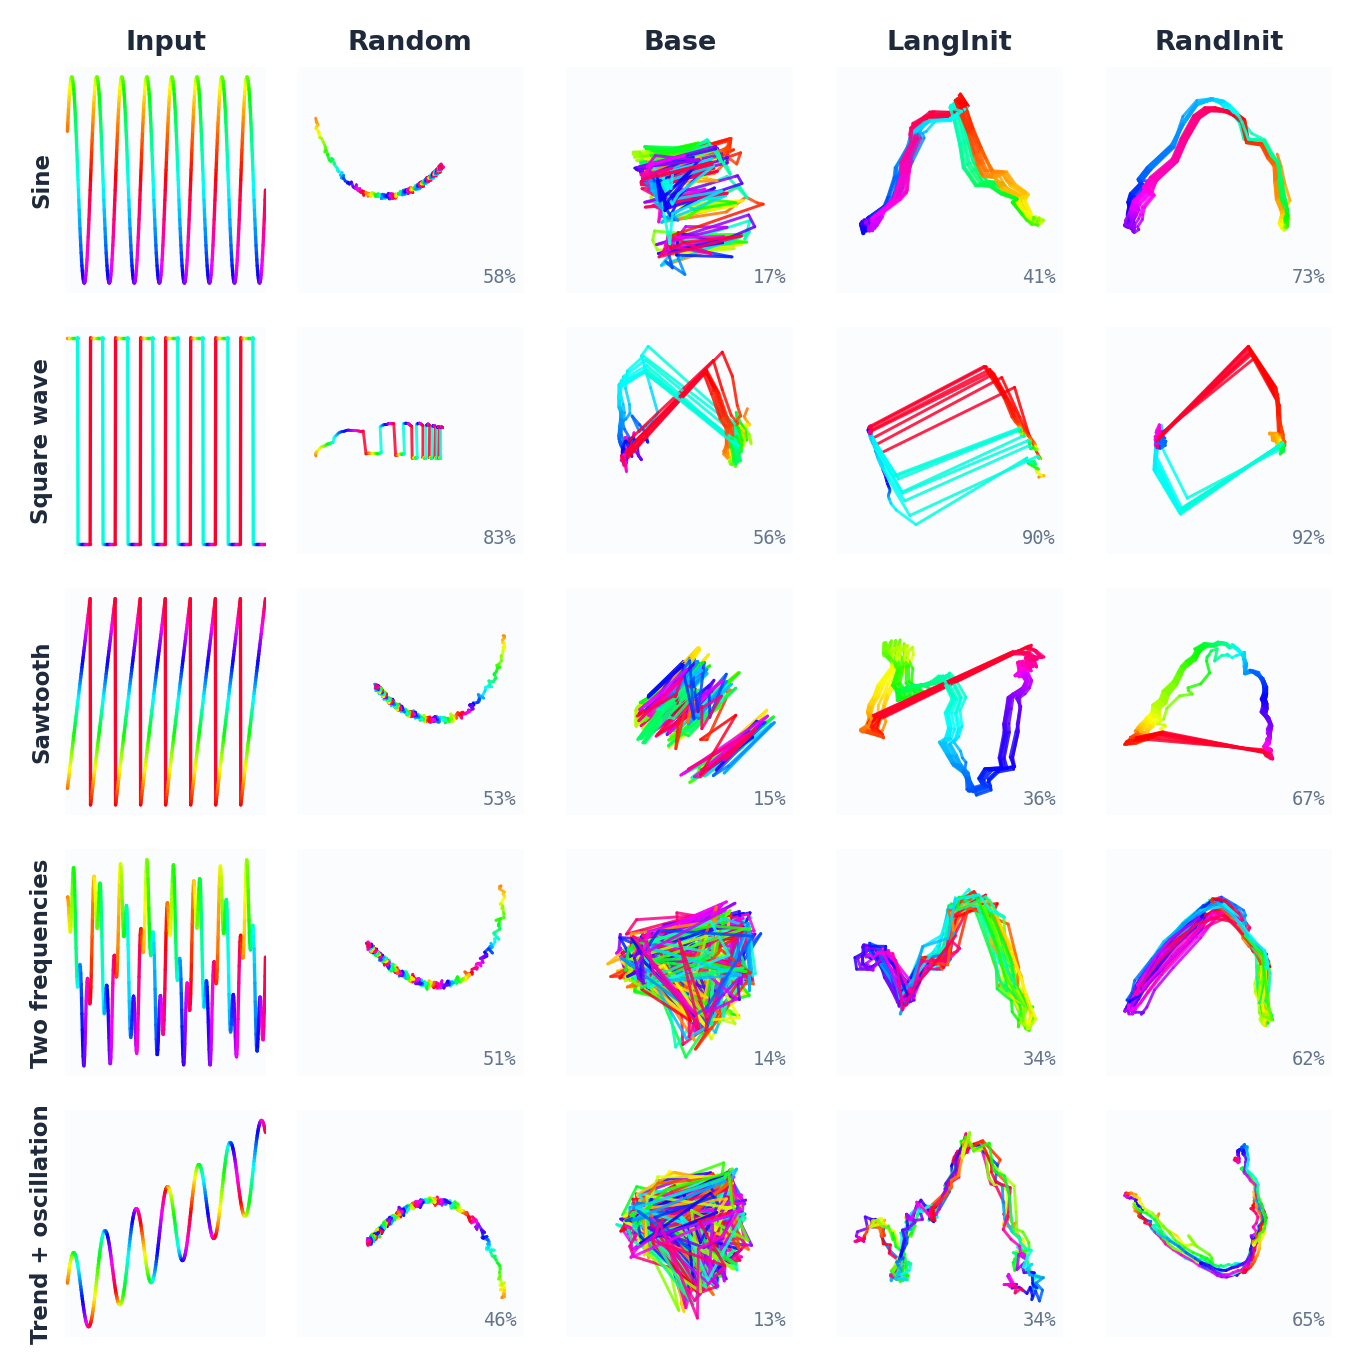
\includegraphics[width=0.85\textwidth]{figures/sec5/fig_synthetic_L13_pca.png}
\caption{\textbf{Hidden-state trajectories for synthetic inputs at Layer~13 (PCA).} Each row is a different input waveform; columns show a randomly initialized untrained model (Random), the pretrained LLM (Base), the language-initialized model finetuned on time series (LangInit), and the randomly-initialized model trained on time series (RandInit). Trajectories are 2D PCA projections of hidden states, colored by input phase. Percentages show variance captured by 2 PCs. Random and Base produce unstructured trajectories. RandInit discovers clean, low-dimensional representations (62--92\% PCA variance) while LangInit creates geometrically complex but structured trajectories (34--98\%) that vary by input type.}
\label{fig:synthetic_pca}
\end{figure}

Figure~\ref{fig:synthetic_pca} extends this analysis to all five synthetic inputs at Layer~13. RandInit consistently produces clean, geometrically simple trajectories with high PCA variance, while LangInit creates more complex structures that vary by input type. Notably, both models arrive at representations that capture the same underlying temporal patterns---the t-SNE projections in Figure~\ref{fig:synthetic_tsne} (Appendix) confirm that the global geometries arrive at the same solution. The key difference is \emph{interpretability}: RandInit's representations are more readily decomposed by linear methods (PCA), whereas LangInit distributes information nonlinearly across more dimensions. The training dynamics of these representations are visualized in Figures~\ref{fig:evolution_grid_ft} and~\ref{fig:evolution_grid_ri} in the Appendix and confirm that pretrained models reuse the complex, high effective rank solutions confirmed in Figure~\ref{fig:erank_dynamics}, while RandInit first simplifies the geometry before increasing complexity (and associatively effective rank) and converging to a solution.

\subsection{Interpreting the Transferred Features}
\label{sec:crosscoder_features}

\paragraph{Method.}
We train one sparse crosscoder per layer with a shared encoder and separate PT/FT decoders. The encoder maps pretrained-model activations on decimal-string time series and finetuned-model activations on binned time series into a shared 4{,}096-dimensional Top-$K$ latent space; PT--FT features are ranked by cross-domain firing balance and probed on WikiText-103.

\begin{table}[h]
\centering
\small
\caption{Examples of shared PT--FT crosscoder features. Shared features concentrate in layers~7--10; the examples below link concrete time-series motifs to coherent WikiText genres. Full examples are in Appendix~\ref{app:crosscoder}.}
\label{tab:crosscoder_features_main}
\begin{tabularx}{\linewidth}{clXX}
\toprule
Layer & Feature & Time-series motif & WikiText motif \\
\midrule
10 & 1712 & magnitude jumps / plateaus & measurements and unit conversions \\
9  & 2469 & volatile regime changes & tropical cyclone narratives \\
7  & 3888 & isolated spikes & timestamped naval battles \\
8  & 2567 & missing / NaN windows & \texttt{<unk>} and incomplete references \\
\bottomrule
\end{tabularx}
\end{table}

Thus, the aligned LangInit subspace is populated by reusable primitives, not just arbitrary low-rank directions. In Appendix~\ref{app:circuit}, we present a preliminary causal circuit analysis that provides additional evidence: zero-ablation identifies a superadditive circuit in Layer~1 (head~L1H4 $\leftrightarrow$ MLP\textsubscript{L1}) that is critical for periodic time-series prediction in FT\textsubscript{IO} and, in the pretrained model, is most important for text with sequential repetitive structure.